\chapter{Análisis marginal y derivadas}
\label{cap:marginal}

\section{Pensar «en el margen»}

Si hay una sola idea que distingue al razonamiento económico, es el \textbf{pensamiento marginal}: para decidir si hago \emph{un poco más} de algo, comparo el beneficio adicional con el costo adicional de esa unidad extra. No importa lo que ya gasté (eso es pasado, «costo hundido»); importa qué sumo y qué resto \emph{en el margen}. Mankiw lo enuncia como uno de sus diez principios de la economía: «las personas racionales piensan en términos marginales» \cite{mankiw}.

La herramienta matemática del pensamiento marginal es la \textbf{derivada}. Por eso este capítulo es, a la vez, un repaso de cálculo y una de las claves conceptuales del curso.

\section{La derivada como tasa de cambio}

\begin{definicion}[Derivada]
La \emph{derivada} de una función $f$ en un punto $x$ mide la tasa instantánea a la que $f$ cambia ante un cambio infinitesimal de $x$:
\[
f'(x) = \frac{\dd f}{\dd x} = \lim_{h\to 0}\frac{f(x+h)-f(x)}{h}.
\]
Geométricamente, es la \emph{pendiente} de la recta tangente a la curva en ese punto.
\end{definicion}

La lectura económica es directa: la derivada responde «si aumento $x$ en una unidad pequeña, ¿cuánto cambia $f$?». Recordemos algunas reglas que usaremos sin demostrar (están en cualquier manual de matemática para economistas, p. ej. \cite{sydsaeter}):
\[
\frac{\dd}{\dd q}(q^n) = n\,q^{\,n-1}, \qquad
\frac{\dd}{\dd q}(k) = 0, \qquad
\frac{\dd}{\dd q}\big(u(q)\pm v(q)\big) = u'(q)\pm v'(q).
\]

\section{Costo, ingreso y beneficio marginales}

Aplicando la derivada a las funciones del Capítulo~\ref{cap:funciones} obtenemos las magnitudes marginales:
\begin{align}
\text{Costo marginal:}\quad & \cmg(q) = C'(q) = \frac{\dd C}{\dd q}, \\[3pt]
\text{Ingreso marginal:}\quad & \img(q) = I'(q) = \frac{\dd I}{\dd q}, \\[3pt]
\text{Beneficio marginal:}\quad & \Pi'(q) = \img(q) - \cmg(q).
\end{align}
La última igualdad encierra la regla de oro de la producción: \emph{conviene producir una unidad más mientras el ingreso marginal supere al costo marginal} ($\img > \cmg$), porque esa unidad agrega más de lo que cuesta. El óptimo se alcanza cuando se igualan, $\img = \cmg$, idea que formalizamos en el Capítulo~\ref{cap:optimizacion}.

\begin{ejemplo}[Del costo total al costo marginal]
Sea $C(q) = 50 + 10q + 0.5q^2$. Derivando término a término:
\[
\cmg(q) = C'(q) = 10 + q.
\]
El costo de la primera unidad es aproximadamente $\cmg(1)=11$, y el de la unidad número 20 es $\cmg(20)=30$: el costo marginal crece, reflejando rendimientos decrecientes. Notá que el costo fijo (50) \emph{desaparece} al derivar: lo fijo no afecta la decisión marginal, coherente con la intuición de que los costos hundidos no deben pesar en el margen.
\end{ejemplo}

\section{La relación entre lo marginal y lo medio}

Una propiedad que confunde al principio pero es muy útil: \textbf{el marginal arrastra al medio}. Cuando el valor marginal está por debajo del promedio, el promedio cae; cuando está por encima, el promedio sube; y se cruzan en el mínimo (o máximo) del promedio. Es la misma lógica que las notas: si te sacás en un parcial menos que tu promedio, el promedio baja.

Formalmente, derivando el costo medio $\cme(q)=C(q)/q$ con la regla del cociente:
\begin{equation}
\frac{\dd \cme}{\dd q} = \frac{C'(q)\,q - C(q)}{q^2} = \frac{1}{q}\big(\cmg(q) - \cme(q)\big).
\end{equation}
El signo de esta derivada depende de si $\cmg \gtrless \cme$: el costo medio decrece mientras el marginal esté por debajo y crece cuando lo supera, alcanzando su mínimo justo donde $\cmg = \cme$. Esta es la razón teórica de la típica curva de costo medio en forma de U \cite{nicholson}.

\begin{figure}[htbp]
\centering
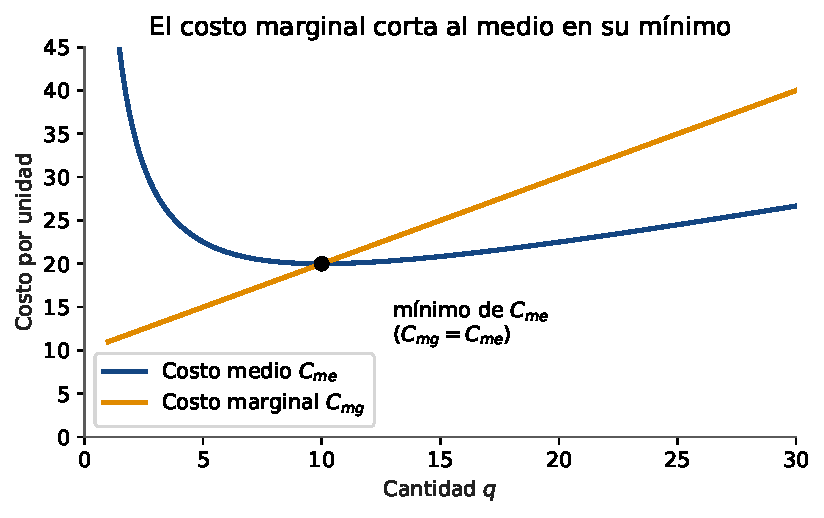
\includegraphics[width=0.72\linewidth]{figuras/costos_U}
\caption{El costo marginal corta al costo medio exactamente en el mínimo de este último: mientras $\cmg<\cme$ el promedio baja; cuando $\cmg>\cme$, sube.}
\label{fig:costos_U}
\end{figure}

\begin{ideabox}
\textbf{Por qué importa para la gestión.} El análisis marginal evita dos errores caros: producir de más (cuando cada unidad nueva cuesta más de lo que rinde) y obsesionarse con costos hundidos. La pregunta correcta nunca es «¿cuánto gasté?», sino «¿qué me suma y qué me cuesta la próxima unidad?».
\end{ideabox}

\begin{labbox}
En el laboratorio, derivar es una sola instrucción: \texttt{sympy.diff(C, q)} devuelve el costo marginal simbólicamente, sin reglas memorizadas. Esto permite obtener $\cmg$, $\img$ y $\Pi'$ a partir de las funciones del capítulo anterior y graficarlas para \emph{ver} dónde el beneficio marginal se hace cero. La computadora hace el cálculo; lo que aporta el economista es saber \emph{qué} derivar y \emph{cómo} interpretarlo.
\end{labbox}

\section{Síntesis del capítulo}

La derivada traduce el pensamiento marginal en cálculo: costo, ingreso y beneficio marginales son derivadas de sus respectivas funciones totales. La relación marginal–medio explica la forma de las curvas de costo. Con la derivada como herramienta de medición del cambio, en el próximo capítulo construimos un concepto que es pura «sensibilidad relativa»: la elasticidad.
